\documentclass[a4paper,12pt]{article}
\usepackage{amsmath,amssymb,amsfonts,amsthm}
\usepackage{tikz}
\usepackage [utf8x] {inputenc}
\usepackage [T2A] {fontenc} 
\usepackage[russian]{babel}
\usepackage{cmap} 
\usepackage{ gensymb }
% Так ссылки в PDF будут активны
\usepackage[unicode]{hyperref}
\usepackage{ textcomp }
\usepackage{indentfirst}
\usepackage[version=3]{mhchem}

% вы сможете вставлять картинки командой \includegraphics[width=0.7\textwidth]{ИМЯ ФАЙЛА}
% получается подключать, как минимум, файлы .pdf, .jpg, .png.
\usepackage{graphicx}
% Если вы хотите явно указать поля:
\usepackage[margin=1in]{geometry}
% Или если вы хотите задать поля менее явно (чем больше DIV, тем больше места под текст):
% \usepackage[DIV=10]{typearea}

\usepackage{fancyhdr}

\newcommand{\bbR}{\mathbb R}%теперь вместо длинной команды \mathbb R (множество вещественных чисел) можно писать короткую запись \bbR. Вместо \bbR вы можете вписать любую строчку букв, которая начинается с '\'.
\newcommand{\eps}{\varepsilon}
\newcommand{\bbN}{\mathbb N}
\newcommand{\dif}{\mathrm{d}}

\newtheorem{Def}{Определение}


\pagestyle{fancy}
\makeatletter % сделать "@" "буквой", а не "спецсимволом" - можно использовать "служебные" команды, содержащие @ в названии
\fancyhead[L]{\footnotesize Квантовая физика}%Это будет написано вверху страницы слева
\fancyhead[R]{\footnotesize ФМХФ МФТИ}
\fancyfoot[L]{\footnotesize \@author}%имя автора будет написано внизу страницы слева
\fancyfoot[R]{\thepage}%номер страницы —- внизу справа
\fancyfoot[C]{}%по центру внизу страницы пусто

\renewcommand{\maketitle}{%
	\noindent{\bfseries\scshape\large\@title\ \mdseries\upshape}\par
	\noindent {\large\itshape\@author}
	\vskip 2ex}
\makeatother
\def\dd#1#2{\frac{\partial#1}{\partial#2}}


\title{5.5 \\ Сцинтилляционная $\gamma$-спектроскопия}
\author{Егор Берсенев} 
\date{16 февраля 2017 г.}

\begin{document}
	
	\maketitle
	\section{Теоретическое введение}
		В данной работе исследуются сцинтилляционные гамма - спектрометры на основе неорганического кристалла NaI(Tl) и органической сцинтиллирующей пластмассы. При прохождении гамма -квантов через материальную среду образуются электроны , возникающие за счет фотоэффекта,  комптоновского рассеяния и рождения  электрон-позитронных пар.
		\subsection{Фотоэффект}
		Процесс взаимодействия $\gamma$-кванта с электроном, связанным с атомом, при котором электрону передается вся энергия гамма-кванта. При этом электрону сообщается кинетическая энергия $T_e = E_\gamma - I_i$. Фотоэффект существенен для тяжелых атомов, где он идет с высокой вероятностью даже при высоких энергиях гамма-квантов.
		\subsection{Эффект Комптона}
		Упругое рассеяние фотона на свободном электроне, сопровождающееся изменением длины волны фотона. Максимальная энергия образующихся комптоновских электронов соответствует рассеянию на 180\degres и равна 
		\begin{equation}
		    E_{max} = \cfrac{\eta\omega}{1+\cfrac{mc^2}{2\eta\omega}}
		\end{equation}
		\subsection{Процесс образования электрон-позитронных пар}
		Образование пары проходит вблизи электрона или ядра. При этом энергия образующегося ядра отдачи оказывается малой, так что энергия образования пары практически совпадает с энергией покоя электрона. Появившийся электрон теряет энергию на ионизацию среды. Таким образом, вся энергия электрона остается в детекторе. Позитрон будет двигаться до тех пор, пока не остановится, а затем аннигилирует с электроном среды, в результате чего появятся два гамма-кванта. Далее есть три варианта развития событий:
		\begin{enumerate}
		    \item оба кванта не вылетают из детектора, и тогда вся энергия первичного гамма-кванта остается в детекторе
		    \item один из родившихся квантов покидает детектор
		    \item оба кванта покидают детектор
		\end{enumerate}
		Таким образом, каждый происходящий процес вносит свой вклад в энергетический спектр излучения.
		
		Энергии пиков максимальных энергий для комптоновского поглощения зависят от энергии пиков полного поглощения как
	\begin{equation}
		E_{max} = \frac{\hbar \omega}{1 + \frac{m_e c^2}{2 \hbar \omega}}
	\end{equation}
	
	Положение пика обратного поглощения вычисляется по формуле
	\begin{equation}
		E = \frac{\hbar \omega}{1 + \frac{2 \hbar \omega}{m_e c^2}}
	\end{equation}
	
	Форма сигнала ФЭУ имеет вид
	\begin{equation}
		U(t) = const \cdot \exp\left(-\frac{t}{RC}\right)\left(1 - \exp\left(-\frac{t}{\tau_0}\right)\right)
	\end{equation}
		
	\section{Эксперимент}
	    Проведем измерения гамма-спектров для всех препаратов:
	    \subsection{$^{60}Co$}
	    
	        \begin{figure}[h!]
	            \centering
12	            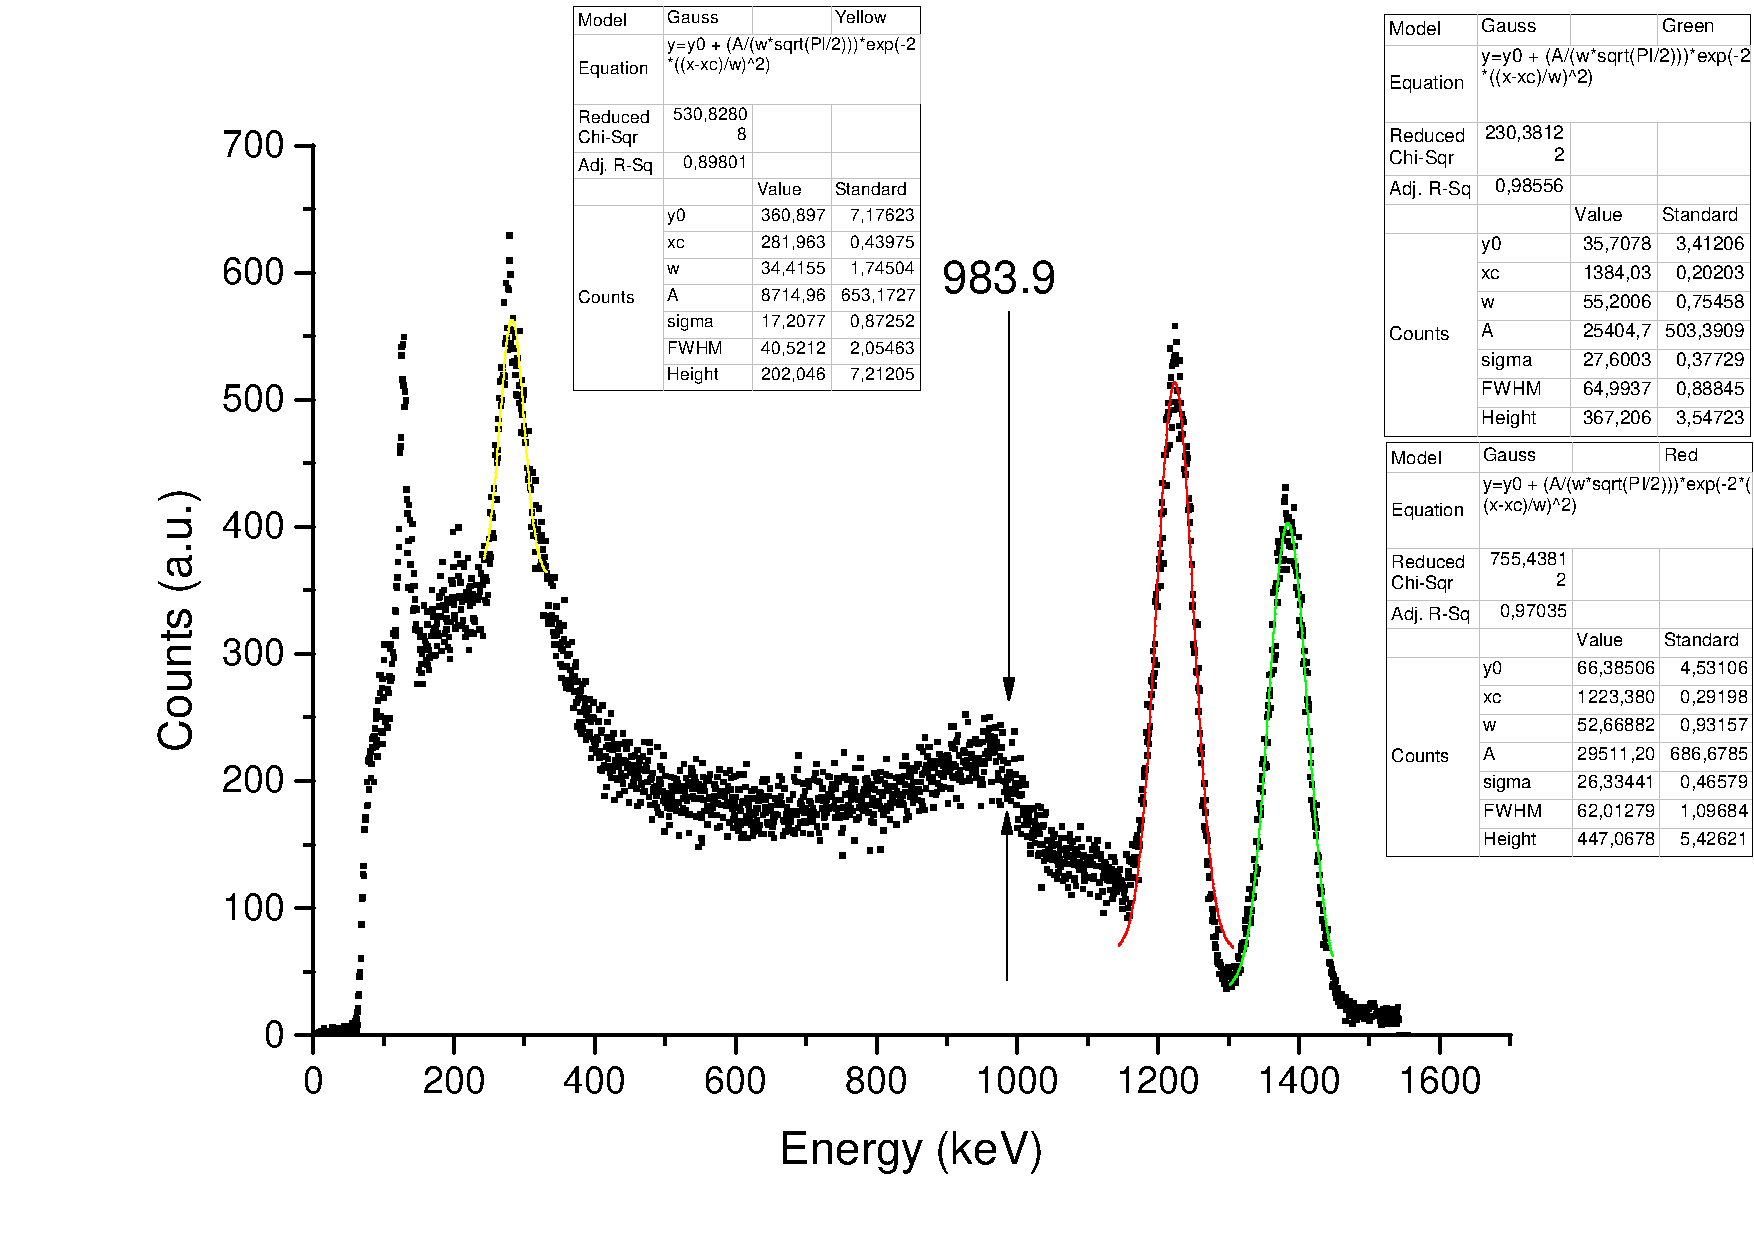
\includegraphics[width=\linewidth]{co60.pdf}
	            \caption{Спектр $^{60}Co$}
	            \label{co60_e}
	        \end{figure}
	        
	        \begin{figure}[h!]
	            \centering
	            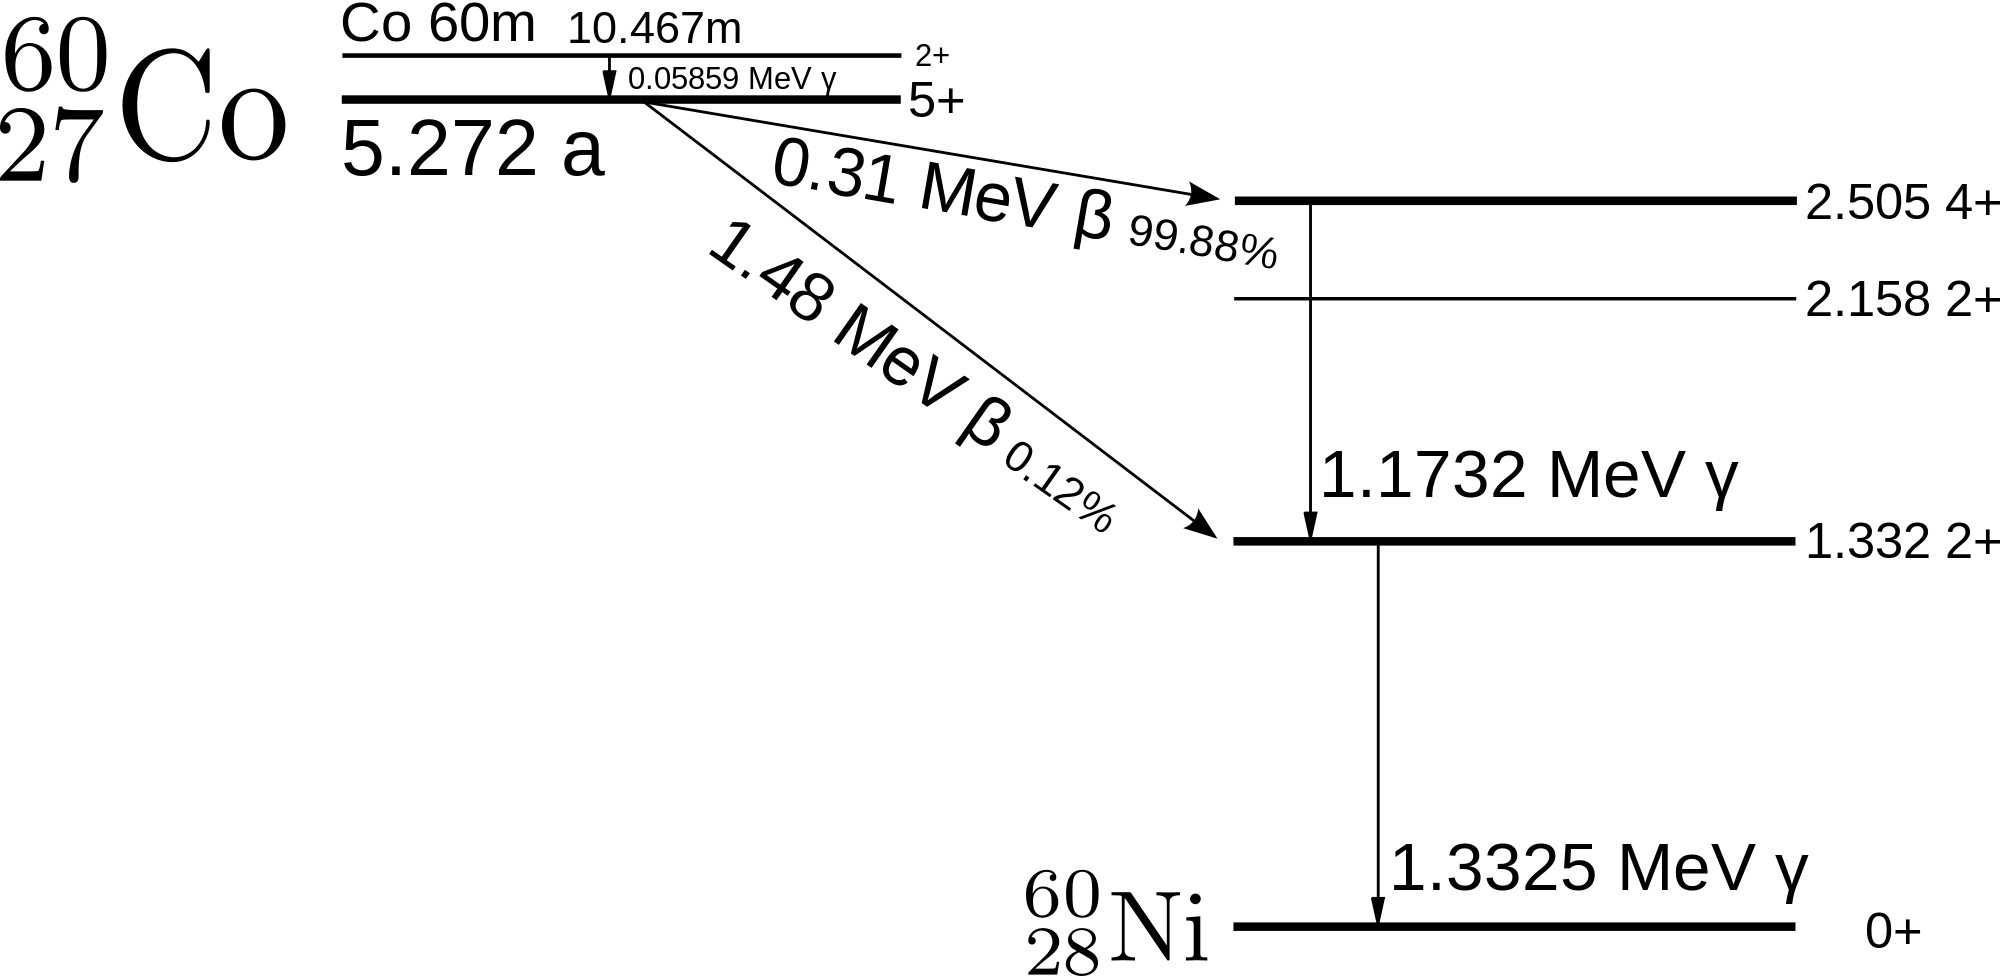
\includegraphics[width=0.4\linewidth]{2000px-Cobalt-60m-decay.png}
	            \caption{Схема распада $^{60}Co$}
	            \label{co60_d}
	        \end{figure}
	       
	   \pagebreak
	        
	   \subsection{$^{137}Cs$}
	    
	        \begin{figure}[h!]
	            \centering
	            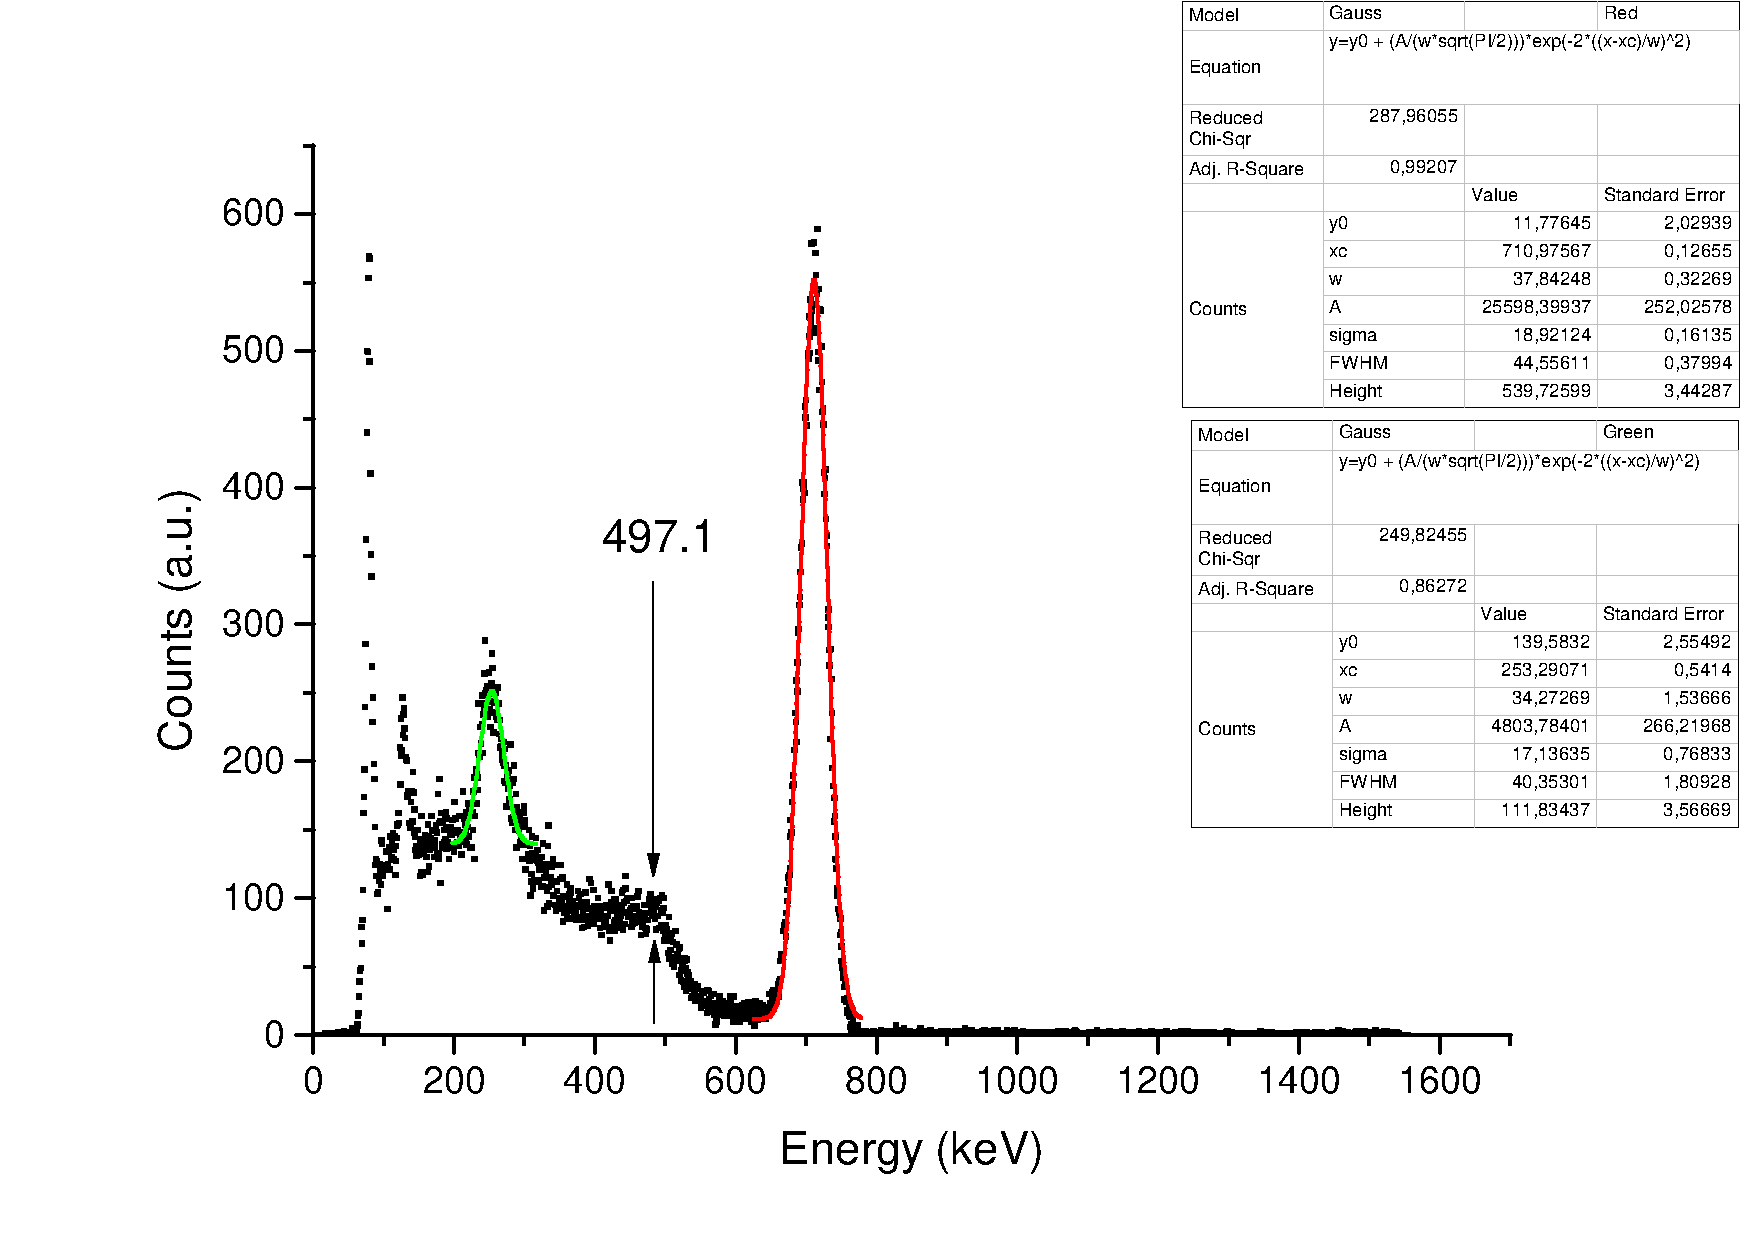
\includegraphics[width=\linewidth]{cs137.pdf}
	            \caption{Спектр $^{137}Cs$}
	            \label{cs137_e}
	        \end{figure}
	        
	        \begin{figure}[h!]
	            \centering
	            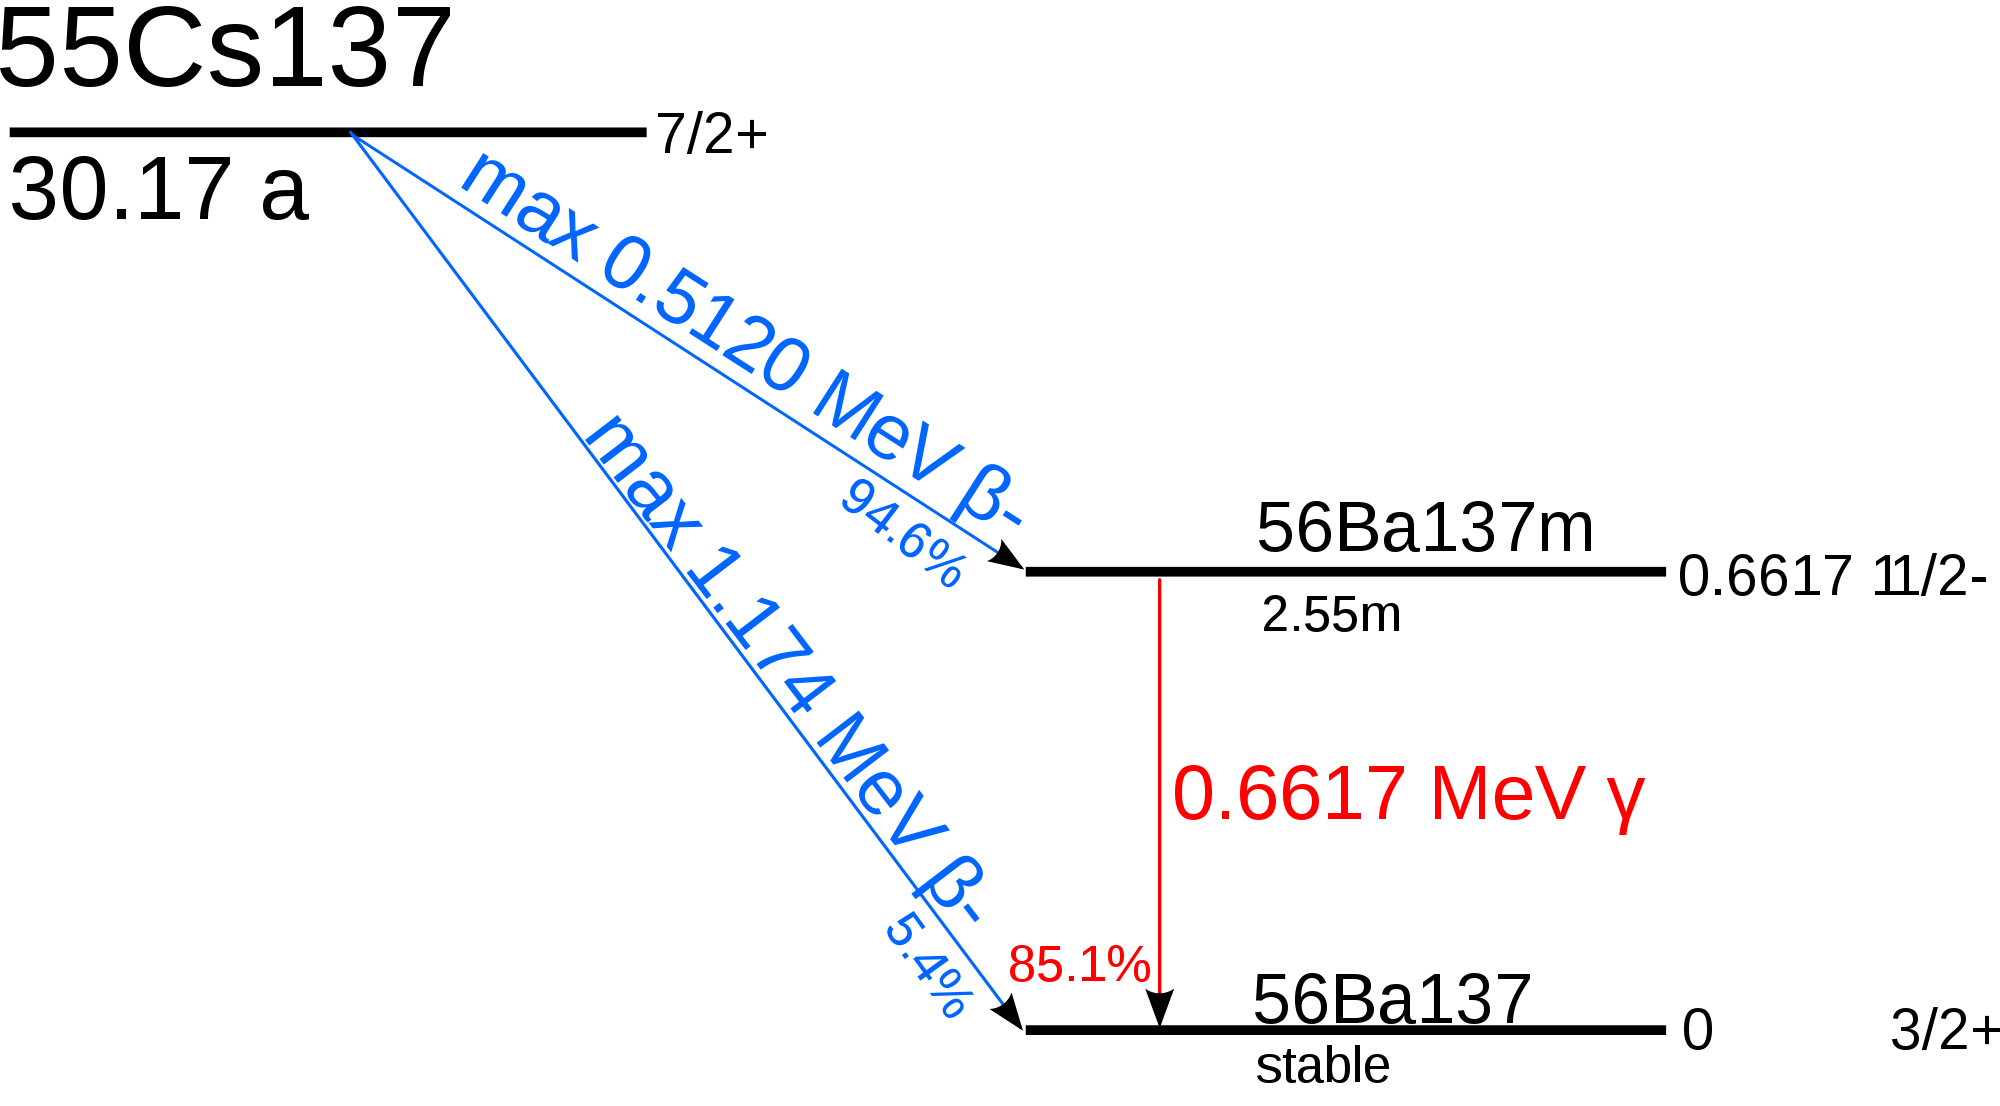
\includegraphics[width=0.4\linewidth]{2000px-Cs-137-decay.png}
	            \caption{Схема распада $^{137}Cs$}
	            \label{cs137_d}
	        \end{figure}
	       
	   \pagebreak
	   
	       
	   \subsection{$^{152}Eu$}
	    
	        \begin{figure}[h!]
	            \centering
	            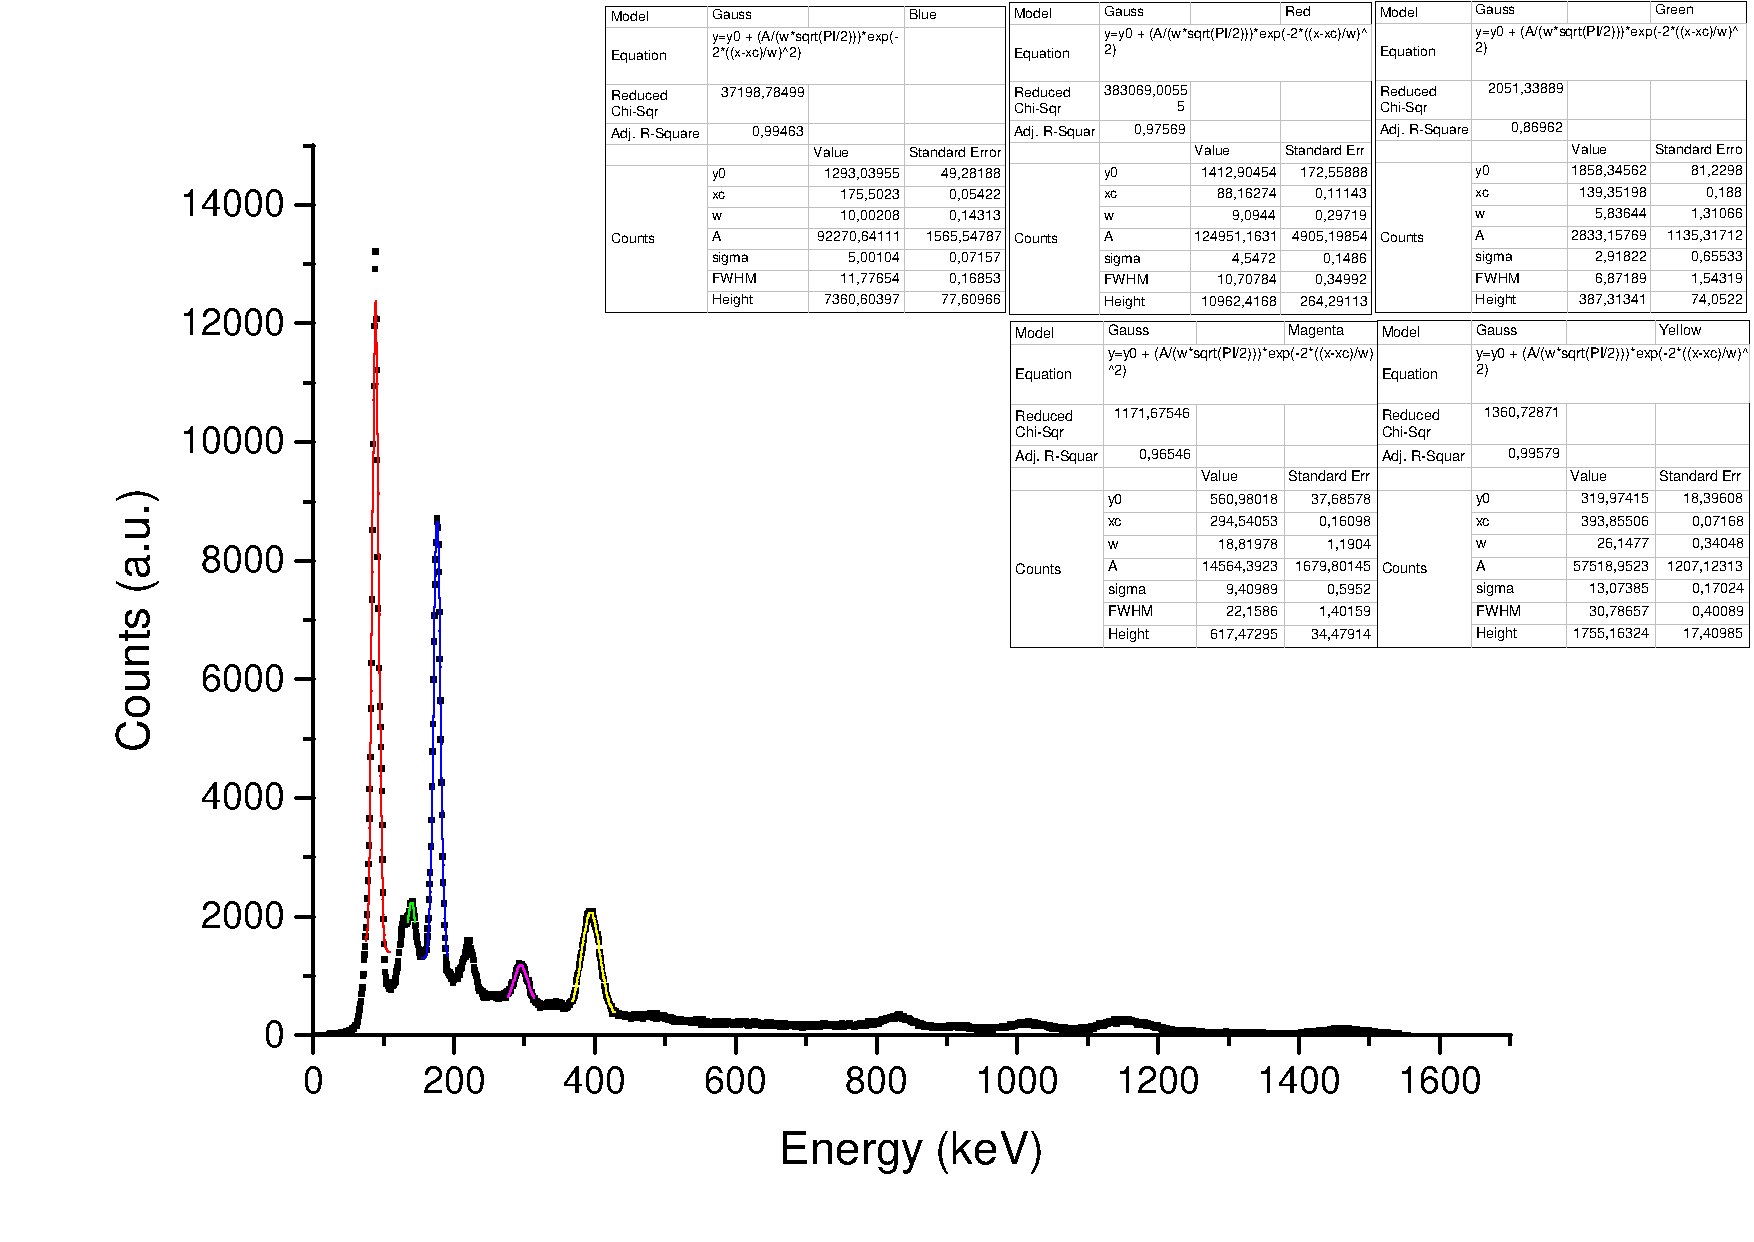
\includegraphics[width=0.8\linewidth]{eu152.pdf}
	            \caption{Спектр $^{152}Eu$}
	            \label{cs137_e}
	        \end{figure}
	        
	        \begin{figure}[h!]
	            \centering
	            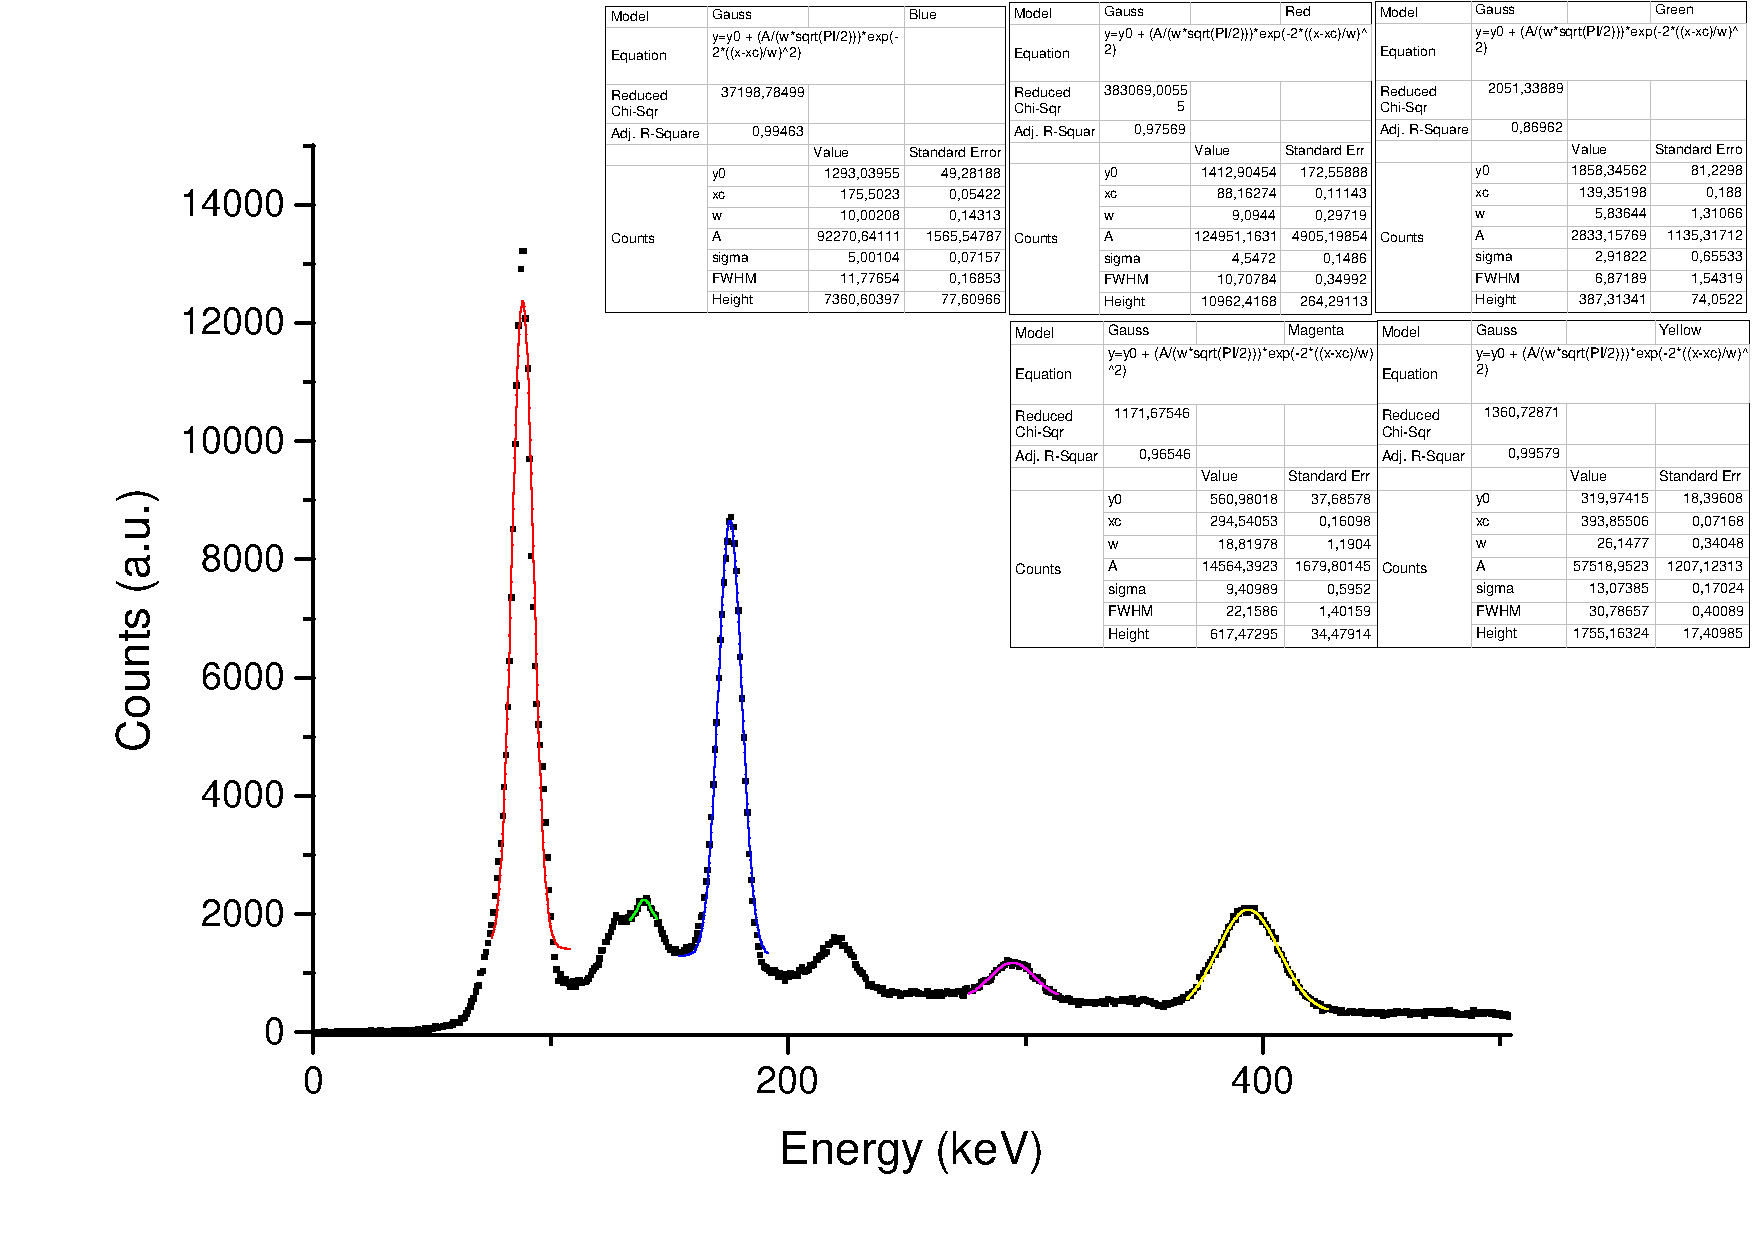
\includegraphics[width=0.8\linewidth]{eu152_enl.pdf}
	            \caption{Спектр $^{152}Eu$}
	            \label{cs137_e}
	        \end{figure}
	        
	        \begin{figure}[h!]
	            \centering
	            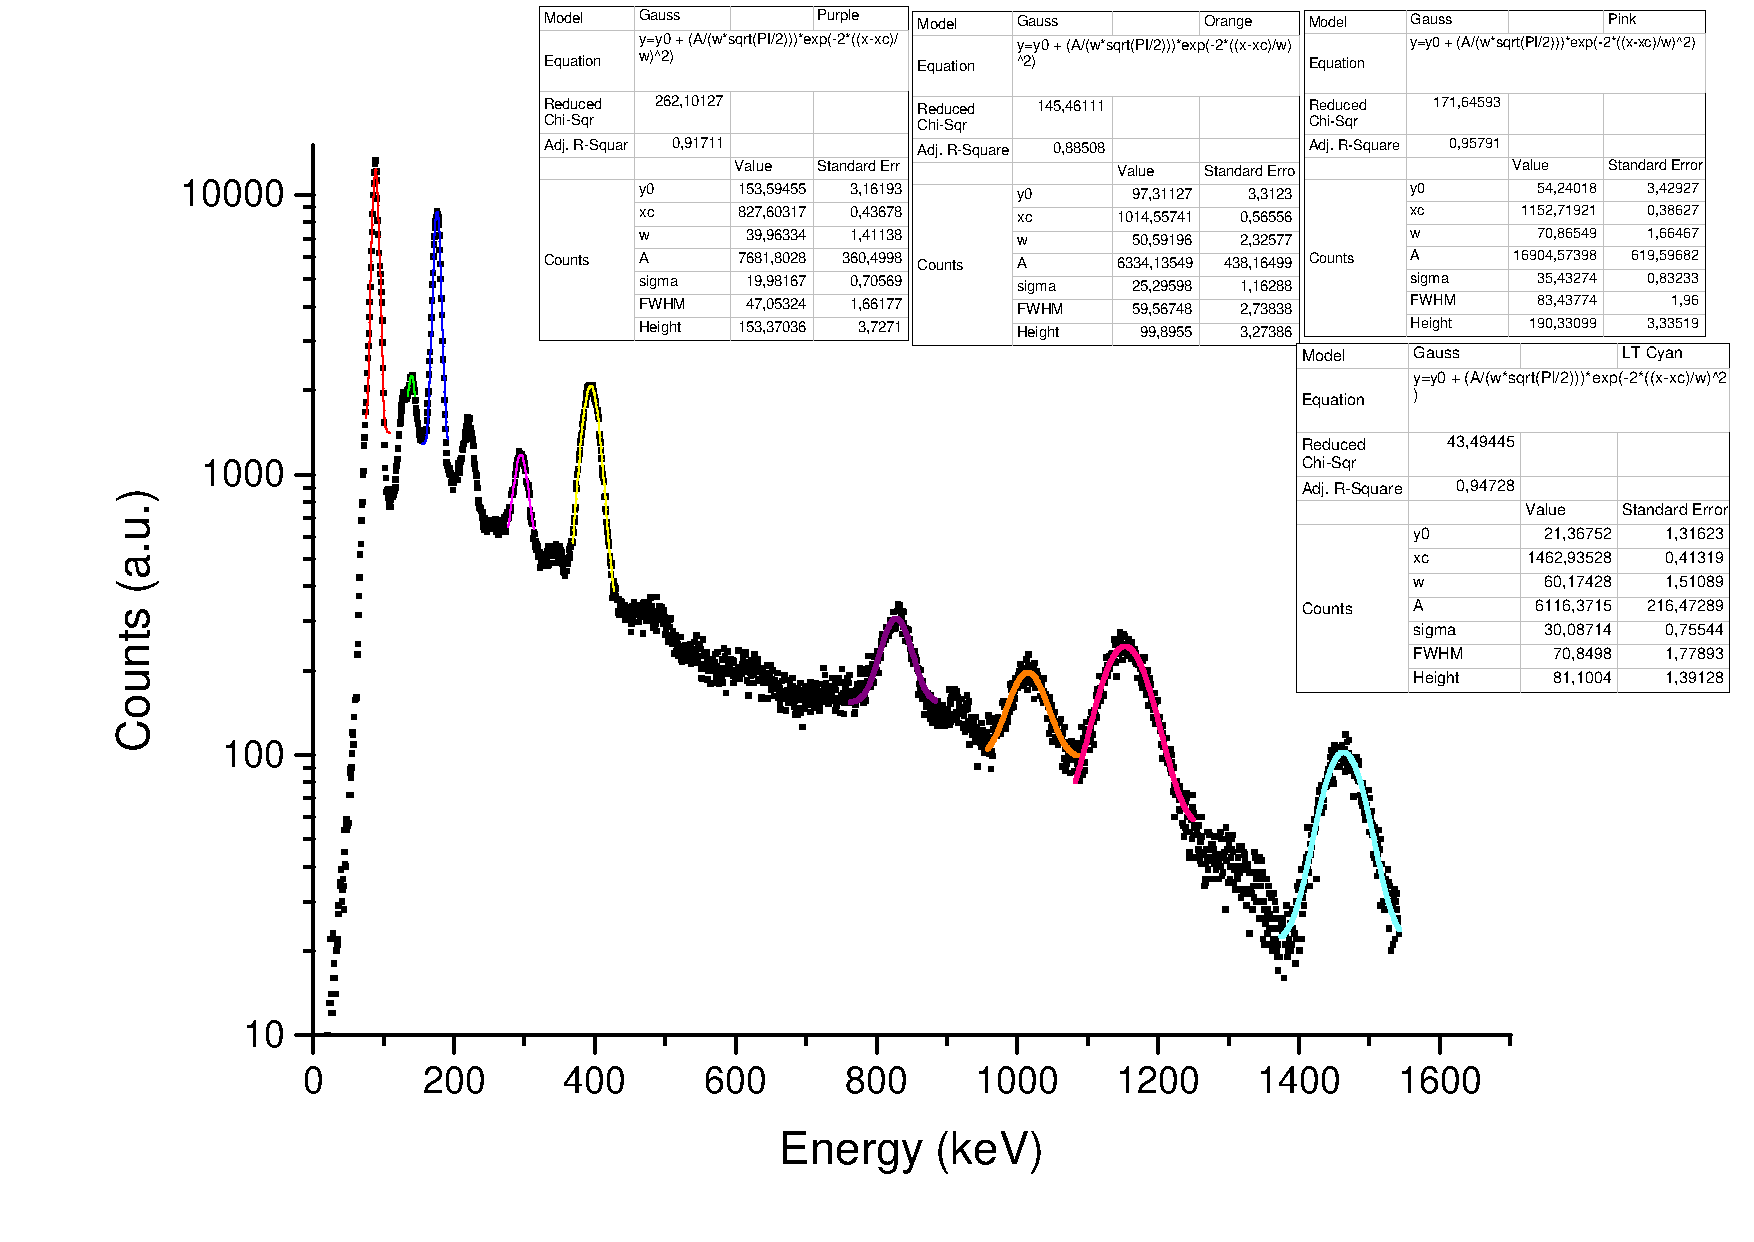
\includegraphics[width=0.8\linewidth]{eu152_log.pdf}
	            \caption{Спектр $^{152}Eu$}
	            \label{cs137_e}
	        \end{figure}
	        
	        \begin{figure}[h!]
	            \centering
	            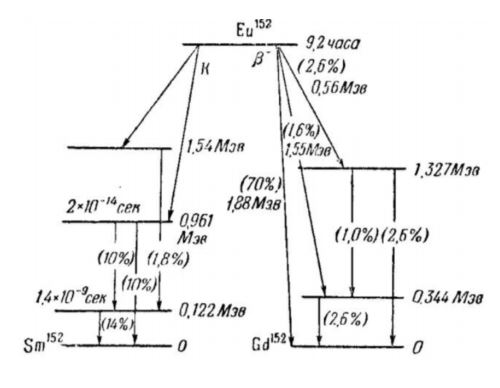
\includegraphics[width=0.4\linewidth]{europium_scheme}
	            \caption{Схема распада $^{152}Eu$}
	            \label{cs137_d}
	        \end{figure}
	        
	  \pagebreak
	  
	  \subsection{$^{22}Na$}
	  
	    \begin{figure}[h!]
	            \centering
	            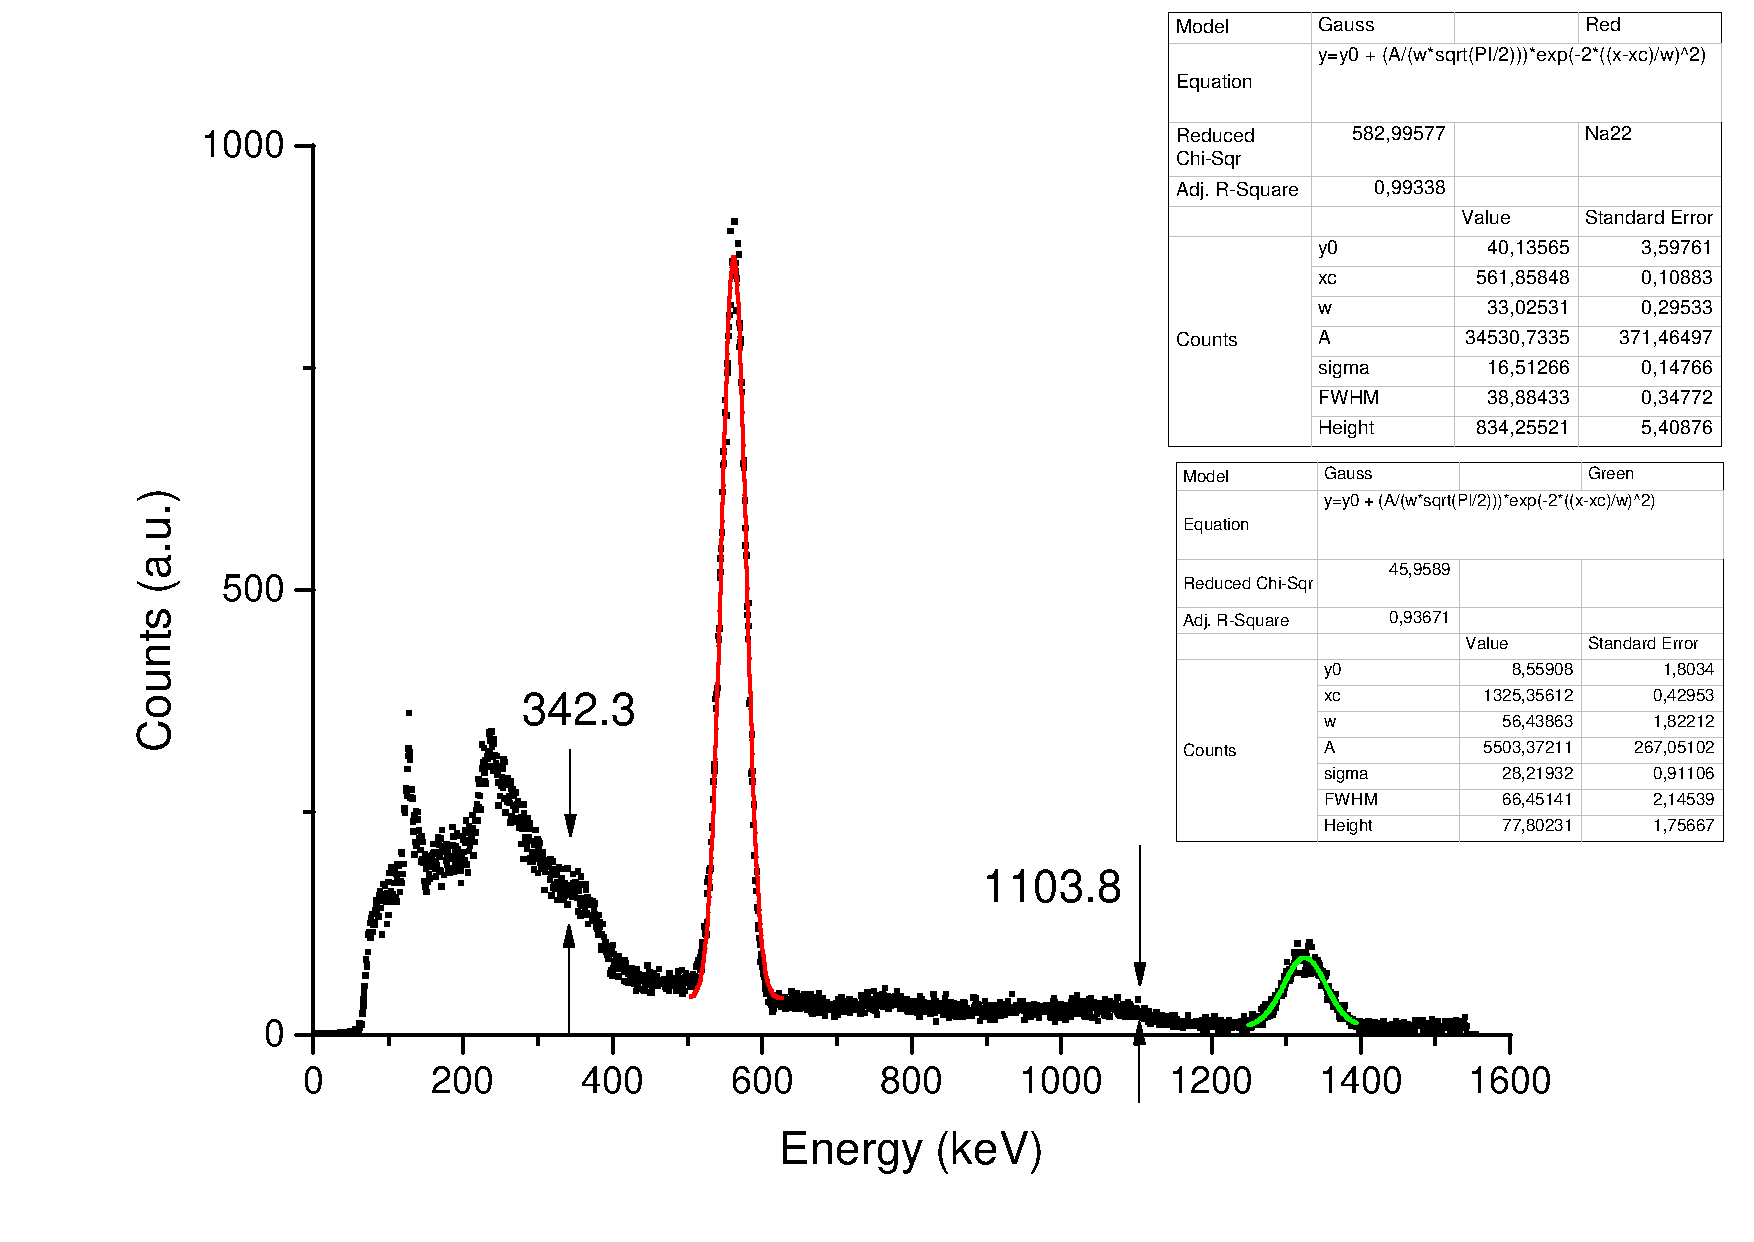
\includegraphics[width=\linewidth]{na22.pdf}
	            \caption{Спектр $^{22}Na$}
	            \label{cs137_e}
	        \end{figure}
	        
	        \begin{figure}[h!]
	            \centering
	            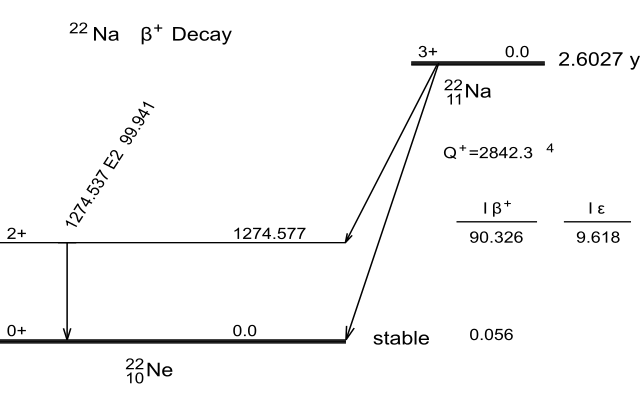
\includegraphics[width=0.4\linewidth]{Na-22_decay_scheme.png}
	            \caption{Схема распада $^{22}Na$}
	            \label{cs137_d}
	        \end{figure}
	        
	        
	    \pagebreak
	        
	   \subsection{$^{241}Am$}
	  
	    \begin{figure}[h!]
	            \centering
	            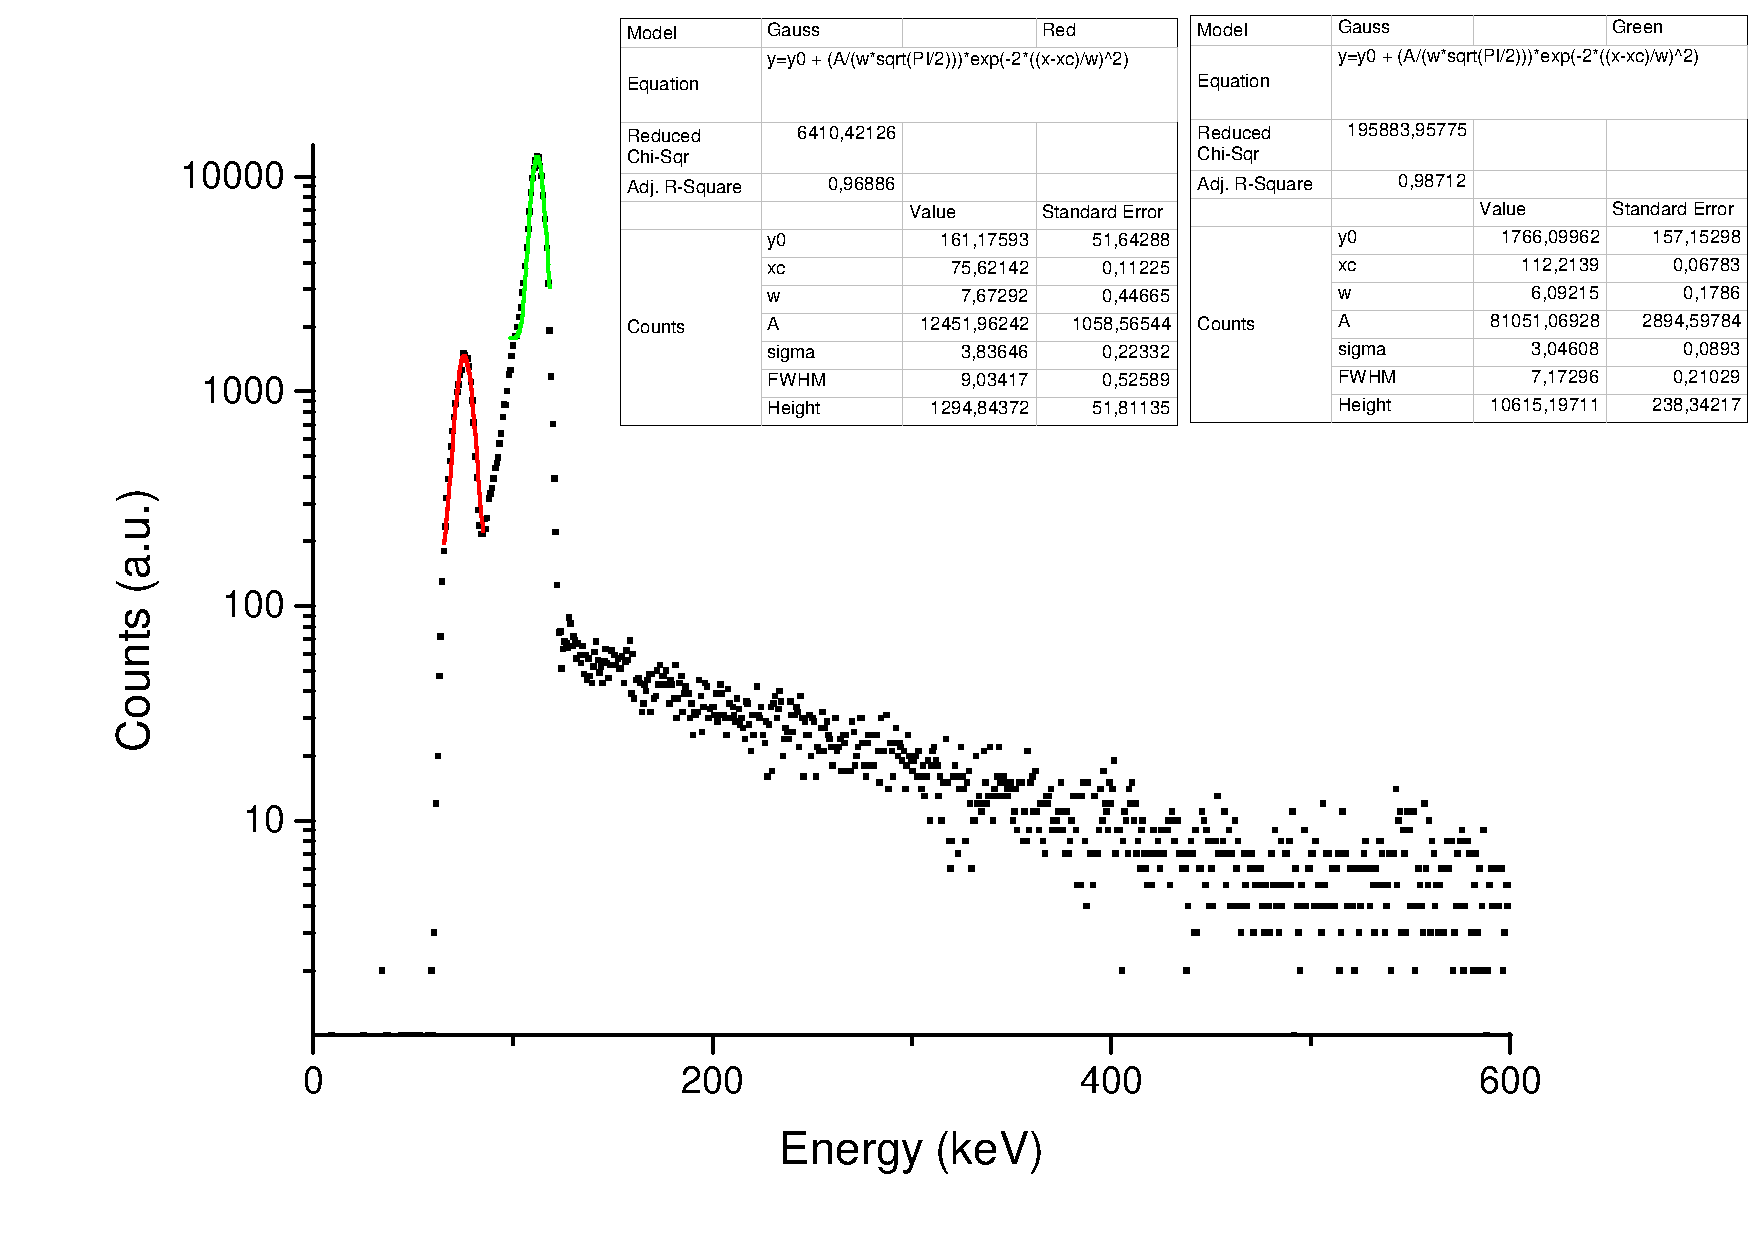
\includegraphics[width=\linewidth]{am241.pdf}
	            \caption{Спектр $^{241}Am$}
	            \label{cs137_e}
	        \end{figure}
	        
	        \begin{figure}[h!]
	            \centering
	            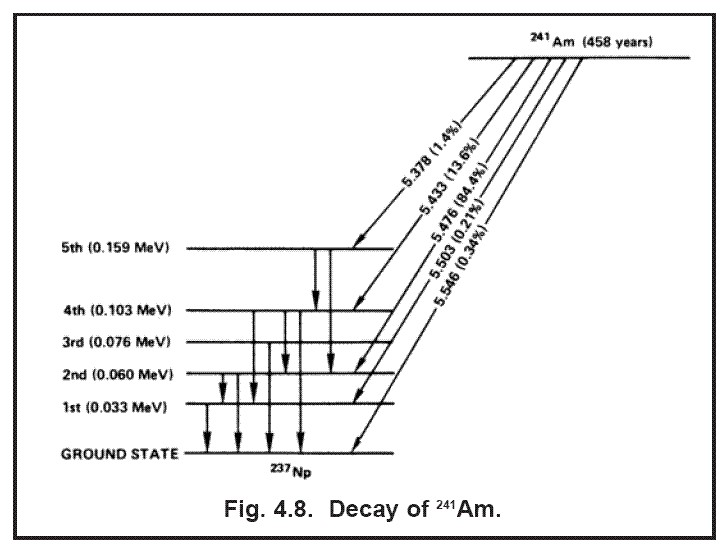
\includegraphics[width=0.4\linewidth]{Am-241_decay.jpg}
	            \caption{Схема распада $^{241}Am$}
	            \label{cs137_d}
	        \end{figure}
	        
	        \newpage
	        
	  Построим график зависимости теоретического значения комптоновского края от экспериментального:
	  
	 \begin{figure}
	     \centering
	     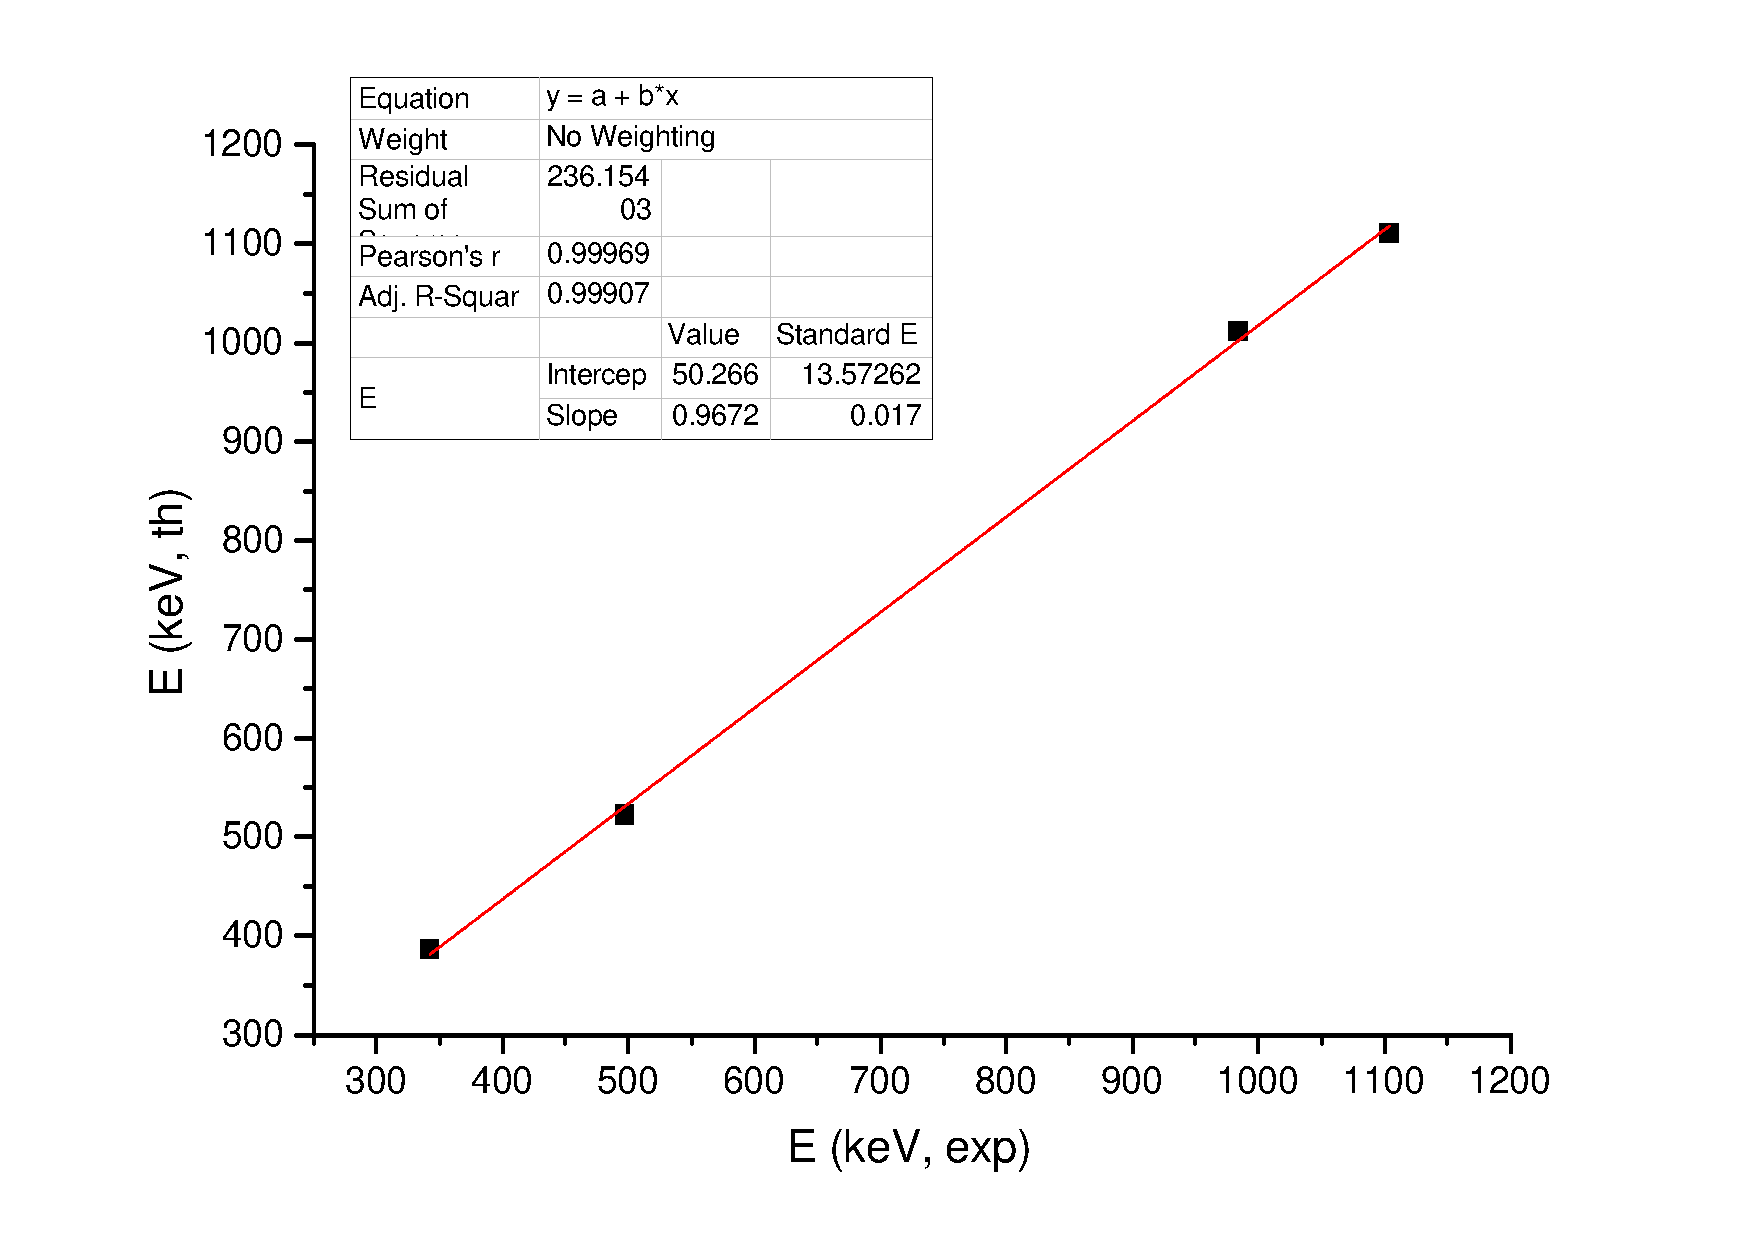
\includegraphics[width=\linewidth]{komp.pdf}
	     \caption{Комптоновские края}
	     \label{fig:my_label}
	 \end{figure}
	 
	 Построим график зависимости энергетического разрешения спектрометра от обратной энергии.
	 
	 \begin{figure}
	     \centering
	     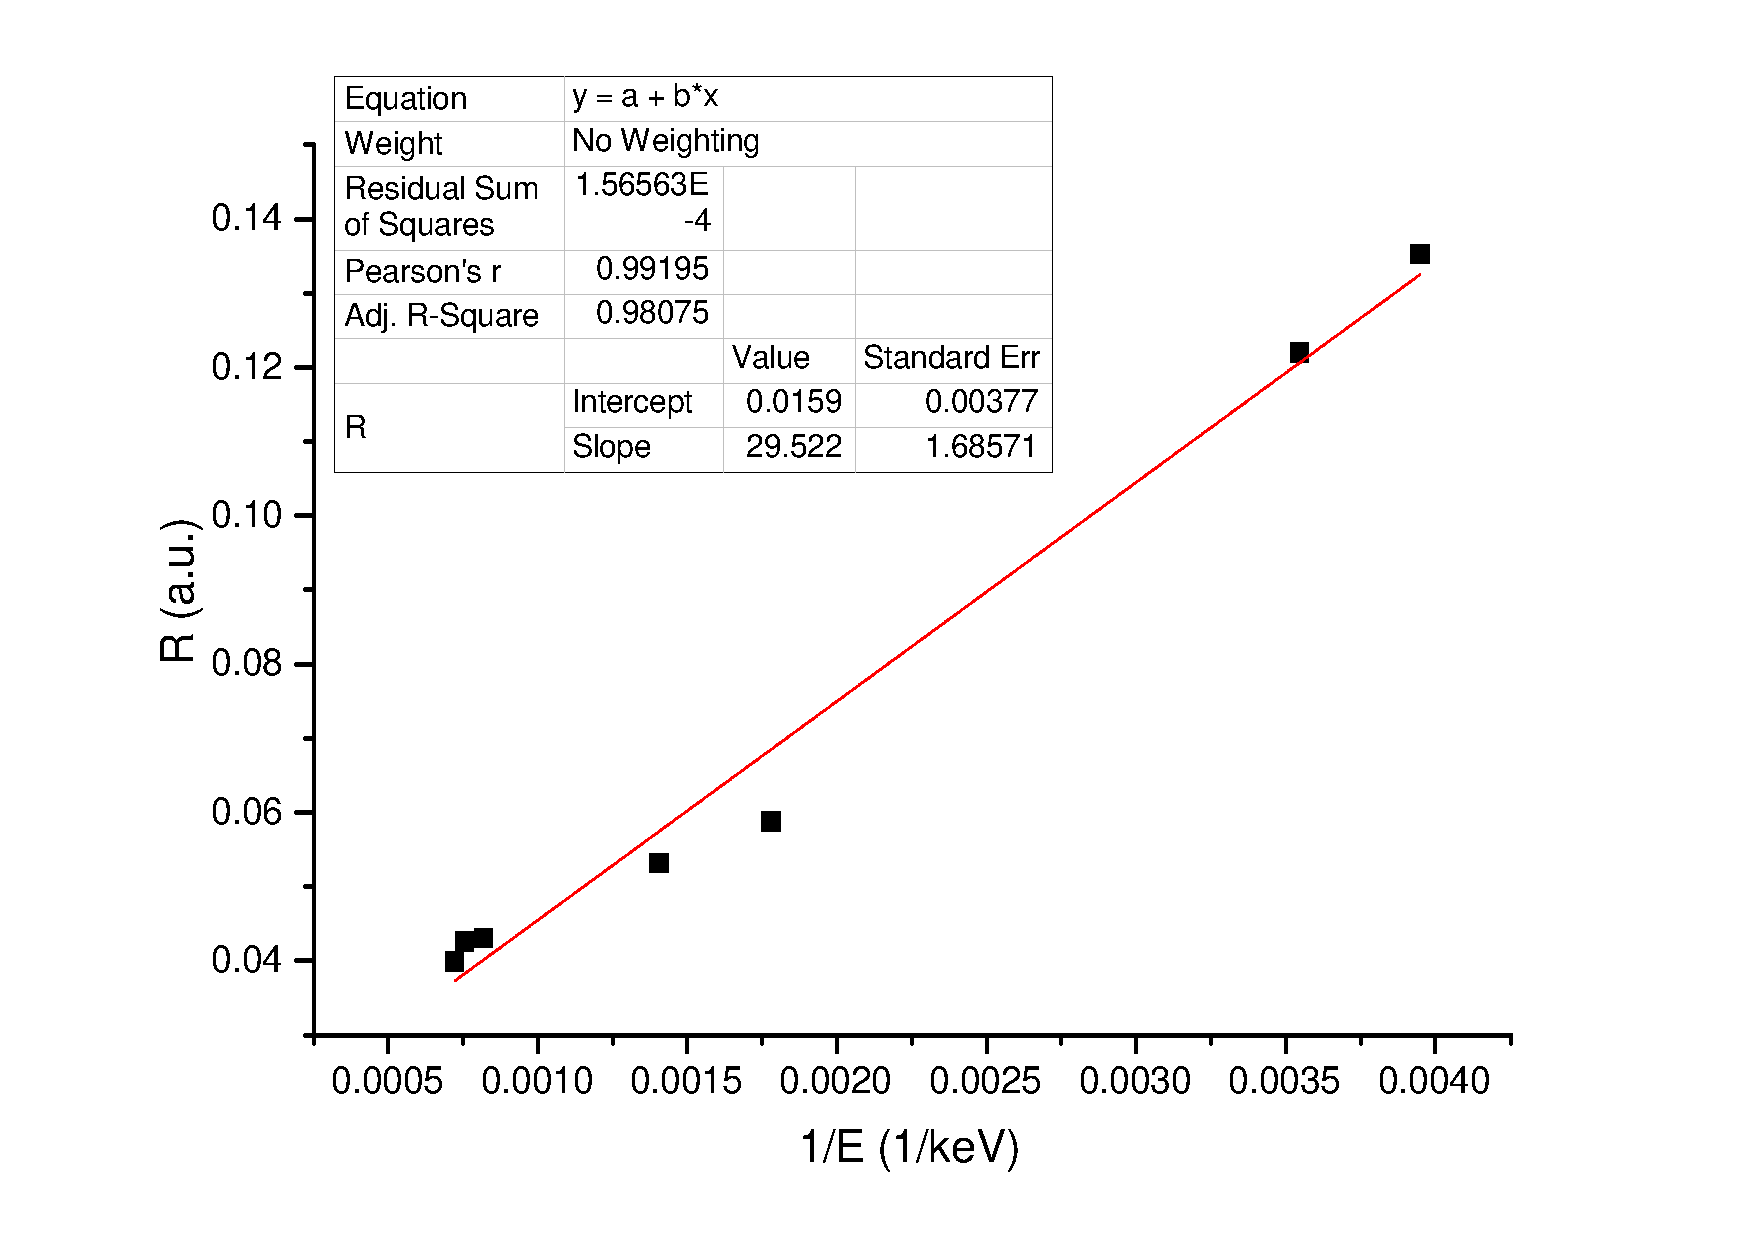
\includegraphics[width=0.8\linewidth]{res.pdf}
	     \caption{Разрешение}
	     \label{fig:my_label}
	 \end{figure}
	 
	 \pagebreak
	 
	 
	 Исследуем постоянную времени и RC-постоянную:
	 \begin{figure}[h!]
	     \centering
	     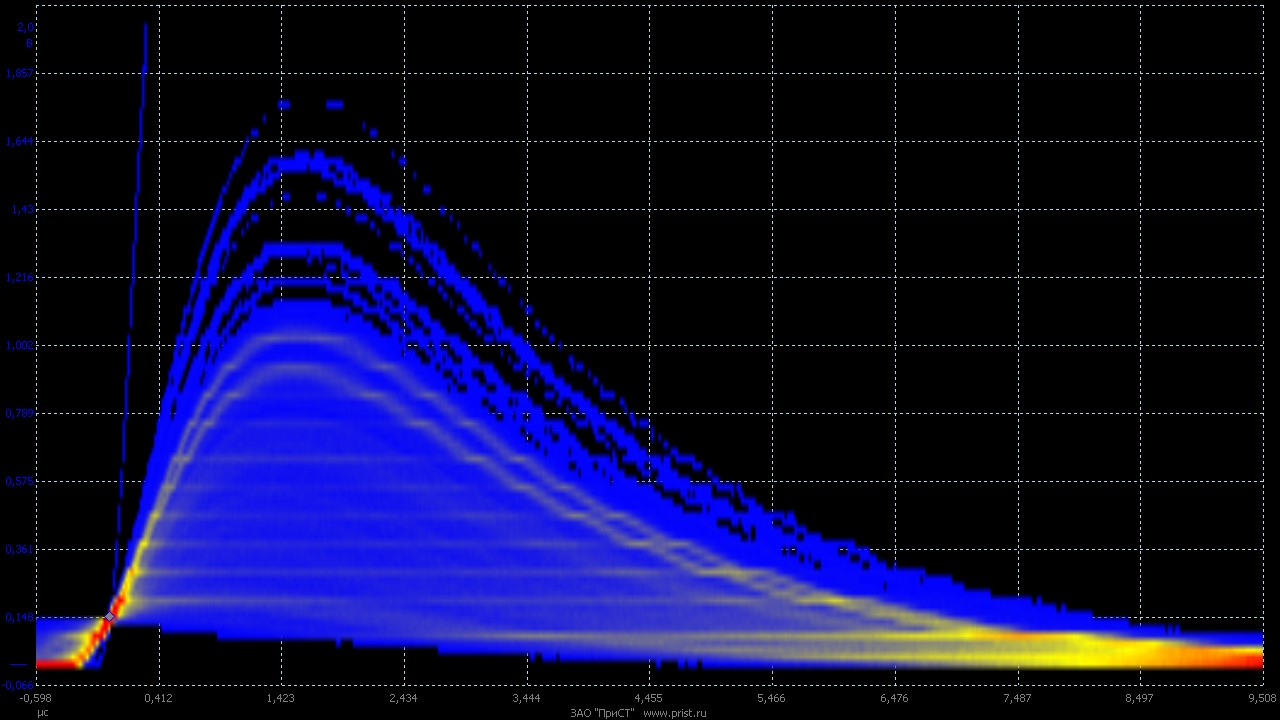
\includegraphics[width=0.8\linewidth]{co_resized}
	     \caption{Форма импульса}
	     \label{fig:my_label}
	 \end{figure}
	 
	 Отсюда $RC\simeq1.5\mu s, \tau \simeq 3.6 \mu s$
	
	
	
	\section{Вывод}
	        
	 	В данной работе был разобран принцип устройства сцинтиллятора. Также был изучен ряд радиоактивных источников и проверены статистические соотношения для разрешающей способности спектрометра.       
	
\end{document}


